\chapter{Experimentos y resultados}
\label{cap:resultados}

Este capítulo presenta los resultados obtenidos con el prototipo y con el modelo de reconocimiento. Las condiciones de evaluación, los esquemas de validación y las métricas se describen en el Capítulo~\ref{cap:metodologia}; el conjunto de datos y el modelo, en el Capítulo~\ref{cap:dataset-modelo}. Todas las cifras provienen de corridas registradas y reproducibles: cada tabla se regenera a partir de los archivos de resultados del repositorio de entrenamiento, sin transcripciones manuales. La interpretación de los resultados se reserva para el Capítulo~\ref{cap:discusion}.

Salvo indicación en contrario, los porcentajes se informan como media $\pm$ desvío estándar entre cinco repeticiones del entrenamiento con semillas distintas.

\section{Desempeño del modelo según el esquema de validación}
\label{sec:res-escenarios}

El conjunto de evaluación reúne 1409 muestras de 13 clases (las 12 señas del vocabulario y la clase «nada»): 1091 provienen de la cámara web de la autora y 318 de la sesión de captura con teléfonos y tabletas de tres personas (P1, P2 y P3). Se excluyeron 109 muestras con menos de cinco cuadros válidos.

La Tabla~\ref{tab:escenarios} compara el mismo problema bajo cinco esquemas de evaluación. Cada uno responde una pregunta distinta: desde cuánto acertaba el modelo con el que comenzó el trabajo sobre tomas reales de los dispositivos, hasta cuánto se infla la medición si las tomas de una misma persona y sesión quedan a ambos lados de la partición.

\begin{table}[h]
    \centering
    \small
    \small
    \begin{tabular}{p{4.6cm}p{5.0cm}rr}
        \toprule
        Esquema & Qué mide & Accuracy (\%) & F1 macro (\%) \\
        \midrule
        Modelo original de la aplicación & solo cámara web, características v1; sobre las tomas de los dispositivos & 28,5 & 25,6 \\
        Solo cámara web, características v2 & mismo entrenamiento, preprocesamiento corregido & 56,0 $\pm$ 5,4 & 53,3 $\pm$ 5,3 \\
        Persona no vista (LOPO) & entrena sin la persona evaluada & 67,3 $\pm$ 2,3 & 67,3 $\pm$ 2,3 \\
        Sesión no vista & agrupado por sesión de grabación & 78,0 $\pm$ 7,1 & 75,1 $\pm$ 7,9 \\
        Esquema anterior (estratificado) & tomas mezcladas al azar; todas las tomas & 94,3 $\pm$ 0,4 & 92,1 $\pm$ 0,5 \\
        \quad sobre las tomas de los dispositivos & las mismas 318 tomas que LOPO & 81,4 & 81,6 \\
        \bottomrule
    \end{tabular}
    \caption{Desempeño del modelo según el esquema de validación (cinco semillas; el $\pm$ es el desvío entre semillas). Salvo el estratificado sobre todas las tomas, que incluye las 1091 de la cámara web, todas las filas se evalúan sobre las tomas de los dispositivos. En una clasificación de una sola etiqueta, el F1 micro coincide con la accuracy.}
    \label{tab:escenarios}
\end{table}

El esquema estratificado, que mezcla al azar las tomas de una misma persona y sesión, informa 94,3\,\%, pero esa cifra se calcula sobre todas las tomas, en su mayoría de la cámara web, que el modelo reconoce casi sin error (98,0\,\%). Sobre las mismas 318 tomas de los dispositivos con las que se evalúa la persona no vista, el esquema estratificado acierta el 81,4\,\%, y LOPO, el 67,3\,\%. Esa diferencia de 14 puntos, medida sobre la misma población, es la que cuantifica cuánto sobreestimaba el esquema anterior la capacidad del modelo de generalizar a personas nuevas.

El desvío del 2,3 de LOPO es entre semillas. Entre personas, el acierto va de 60,0\,\% a 73,0\,\% (desvío de 6,6 puntos; Tabla~\ref{tab:por-persona}): la variación que experimentaría una persona concreta es mayor que la que sugiere el desvío entre semillas.

El modelo con el que comenzó el trabajo, entrenado solo con la cámara web y con la representación de características original, acierta el 28,5\,\% de las tomas reales de los dispositivos. Al mismo tiempo, muestra en pantalla el 83\,\% de sus predicciones (confianza $\geq 0{,}7$) y acierta solo el 32\,\% de ellas.

La Tabla~\ref{tab:por-persona} detalla el acierto por persona y la Tabla~\ref{tab:f1-por-sena}, el F1 por seña.

\begin{table}[h]
    \centering
    \begin{tabular}{lrr}
        \toprule
        Persona & Modelo original (\%) & Persona no vista (\%) \\
        \midrule
        P1 & 39,6 & 60,0 \\
        P2 & 21,9 & 73,0 \\
        P3 & 24,0 & 68,9 \\
        \bottomrule
    \end{tabular}
    \caption{Acierto por persona: modelo original frente a validación con persona no vista. El modelo original se entrenó con la cámara web de P1, por lo que su 39,6\,\% con P1 no corresponde a una persona nueva; con P2 y P3, que nunca vio, acierta el 21,9 y el 24,0\,\%. En la persona no vista, al excluir a P1 también se excluyen las 1091 tomas de cámara web: su pliegue entrena con 212 tomas, frente a unas 1300 en los otros dos, y su 60,0\,\% mezcla el efecto de la persona con el del tamaño del entrenamiento.}
    \label{tab:por-persona}
\end{table}

\begin{table}[h]
    \centering
    \begin{tabular}{lrr}
        \toprule
        Seña & Modelo original & Persona no vista \\
        \midrule
        hola & 40,0 & 91,3 \\
        adiós & 37,5 & 74,7 \\
        bien & 22,7 & 46,4 \\
        ¿cómo estás? & 48,5 & 56,9 \\
        gracias & 13,8 & 46,9 \\
        E & 25,8 & 50,4 \\
        V & 0,0 & 79,8 \\
        L & 0,0 & 76,3 \\
        I & 0,0 & 78,1 \\
        N & 7,7 & 97,1 \\
        mi nombre es & 29,1 & 48,7 \\
        por favor & 82,1 & 76,8 \\
        nada & --- & 51,9 \\
        \bottomrule
    \end{tabular}
    \caption{F1 por seña (\%). El modelo original no tenía la clase «nada».}
    \label{tab:f1-por-sena}
\end{table}

La Figura~\ref{fig:matriz-confusion} muestra la matriz de confusión del esquema persona no vista, acumulada sobre las cinco semillas (1590 predicciones) y normalizada por fila.

\begin{figure}[h]
    \centering
    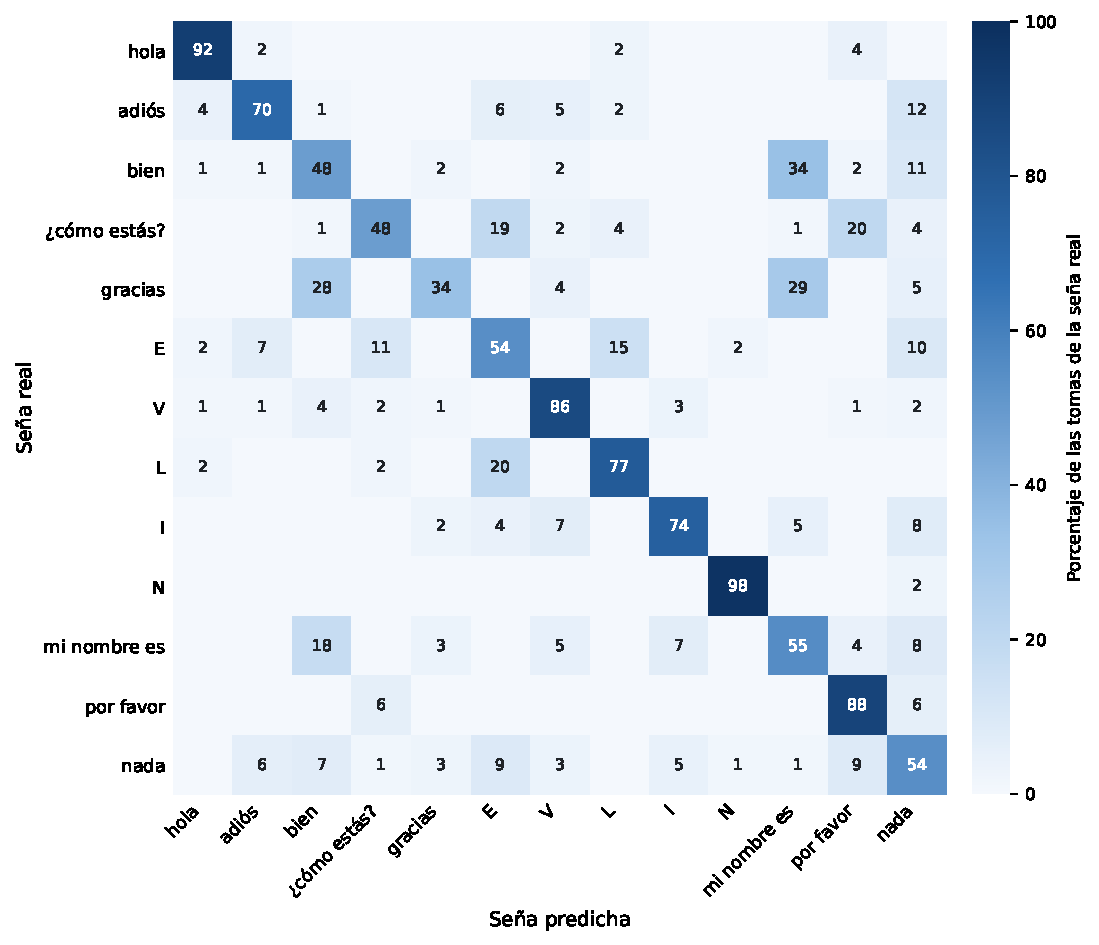
\includegraphics[width=0.92\textwidth]{matriz_confusion_persona.pdf}
    \caption{Matriz de confusión con persona no vista (cinco semillas, 1590 predicciones). Cada fila suma 100\,\%; las celdas vacías no tienen predicciones.}
    \label{fig:matriz-confusion}
\end{figure}

Las señas mejor reconocidas son N (98\,\%), hola (92\,\%), por favor (88\,\%) y V (86\,\%). Las confusiones se concentran en pares de señas con formas o ubicaciones de la mano similares: el 34\,\% de las tomas de «bien» se predice como «mi nombre es» y el 18\,\% de «mi nombre es», como «bien»; «gracias» se confunde con ambas (28\,\% y 29\,\%); «¿cómo estás?» se confunde con «por favor» (20\,\%) y con E (19\,\%), y las letras E y L se confunden entre sí (15\,\% y 20\,\%). La clase «nada» recibe predicciones de casi todas las señas, entre el 2 y el 12\,\% de cada una.

\section{Calibración de la confianza}
\label{sec:res-calibracion}

La confianza que informa el modelo se ajustó mediante escalado de temperatura sobre personas no vistas (nueve pliegues). La temperatura adoptada es $T = 1{,}20$ y reduce el error de calibración esperado (ECE) de 17,1\,\% a 12,7\,\%. La Tabla~\ref{tab:umbral} muestra, para distintos umbrales de confianza calibrada, qué fracción de las predicciones se muestra en pantalla y cuántas de ellas son correctas.

\begin{table}[h]
    \centering
    \begin{tabular}{rrr}
        \toprule
        Umbral & Predicciones mostradas (\%) & Acierto de lo mostrado (\%) \\
        \midrule
        0,70 & 62,9 & 80,8 \\
        0,75 & 59,6 & 83,0 \\
        0,80 & 55,7 & 84,4 \\
        0,85 & 49,7 & 87,1 \\
        \bottomrule
    \end{tabular}
    \caption{Cobertura y acierto según el umbral de confianza calibrada (persona no vista).}
    \label{tab:umbral}
\end{table}

En la aplicación se adoptó el umbral 0,75, algo menor que el 0,85 que sugería el criterio de lograr un 85\,\% de acierto, para mostrar más predicciones: se muestra el 59,6\,\% y se acierta el 83,0\,\% de lo mostrado, frente al 83\,\% mostrado con 32\,\% de acierto del modelo original.

Las cifras de la Tabla~\ref{tab:umbral} son optimistas: el umbral se eligió observando las mismas predicciones sobre las que se informa su acierto. Para medirlo sin ese sesgo se repitió el procedimiento completo, guardando las predicciones, y se evaluó cada persona con un umbral elegido solo a partir de las otras dos. Con el criterio del 85\,\%, el acierto de lo mostrado en la persona excluida fue de 83,5\,\% en promedio, entre 75,9\,\% y 93,1\,\% según la persona, mostrando el 46\,\% de las predicciones. Con el umbral fijo de la aplicación, fue de 72,7\,\%, 81,0\,\% y 86,9\,\% para P1, P2 y P3 (80,2\,$\pm$\,7,1 entre personas). La repetición también mostró la variabilidad del propio procedimiento: el entrenamiento en GPU no es determinista y la temperatura resultó 1,29 en lugar de 1,20. La aplicación conserva la temperatura y el umbral originales, y el acierto que cabe esperar de lo que muestra es de alrededor del 80\,\%, con una variación importante entre personas.

\section{Consistencia estadística}
\label{sec:res-consistencia}

La métrica de consistencia $\sigma$ definida en la propuesta mide si entradas parecidas reciben salidas parecidas, sin utilizar etiquetas (la definición y las decisiones de implementación se presentan en el Capítulo~\ref{cap:metodologia}). Se calculó sobre las 449 tomas de los dispositivos, con un umbral de vecindad $\varepsilon = 0{,}72$: el mayor percentil de las distancias de la sesión~1 para el cual al menos el 90\,\% de los vecinos corresponde a la misma seña (98,4\,\%).

\begin{table}[h]
    \centering
    \begin{tabular}{lrrr}
        \toprule
        Condición & Tomas & Acierto (\%) & $\sigma$ \\
        \midrule
        Estándar (sesión 1) & 318 & 95,3 & 0,008 \\
        Cerca & 36 & 83,3 & 0,008 \\
        Poca luz & 36 & 83,3 & 0,024 \\
        Lejos & 24 & 79,2 & 0,028 \\
        Lejos y poca luz & 12 & 75,0 & 0,036 \\
        Girado 30° & 23 & 56,5 & --- \\
        \bottomrule
    \end{tabular}
    \caption{Consistencia $\sigma$ del modelo publicado en la aplicación, por condición. A 30° solo una de las 23 tomas tiene vecinos dentro de $\varepsilon$.}
    \label{tab:sigma}
\end{table}

La Tabla~\ref{tab:sigma} muestra que $\sigma$ crece en las condiciones adversas: se multiplica por tres con poca luz y por cuatro y medio cuando se combinan distancia y poca luz. Las tomas con el cuerpo girado 30° casi no tienen vecinos en el espacio de entrada, es decir, caen lejos de todas las demás.

Las tomas que el modelo clasifica mal tienen un $\sigma_i$ entre tres y cuatro veces mayor que las que clasifica bien: 0,028 frente a 0,007 en la sesión~1 y 0,052 frente a 0,019 con poca luz.

Con modelos que no vieron a la persona evaluada, $\sigma$ es de dos a cuatro veces mayor (0,022 en la sesión~1, con 67,2\,\% de acierto; es el mismo esquema LOPO de la Tabla~\ref{tab:escenarios}, con tres semillas en lugar de cinco). La métrica depende del umbral elegido: en la sesión~1, $\sigma$ pasa de 0,008 con $\varepsilon = 0{,}72$ a 0,127 con $\varepsilon = 2{,}19$, valor para el cual solo el 30,5\,\% de los vecinos corresponde a la misma seña.

\section{Robustez ante condiciones de captura}
\label{sec:res-robustez}

La segunda sesión de captura registró las doce señas una vez en cada una de cuatro condiciones adversas: poca luz, cerca de la cámara (unos 40\,cm), lejos (unos 120\,cm) y con el cuerpo girado 30°. Las tomas de P3 en la condición «lejos» se grabaron además con poca luz, y se analizan aparte. Las tomas de P3 a 30° se descartaron durante la grabación por problemas de detección, y a P2 le falta una toma a 30°.

Cada condición se compara con su referencia estándar usando el mismo modelo, en dos escenarios: persona no vista (el modelo no conoce a la persona) y persona conocida en una sesión nueva (el modelo conoce a la persona, pero no esa sesión). La Tabla~\ref{tab:robustez} resume los resultados y la Figura~\ref{fig:robustez} los representa con sus intervalos de confianza.

\begin{table}[h]
    \centering
    \small
    \begin{tabular}{lrrrr}
        \toprule
        & \multicolumn{2}{c}{Persona no vista} & \multicolumn{2}{c}{Persona conocida} \\
        Condición & Acierto (\%) & Caída (pts) & Acierto (\%) & Caída (pts) \\
        \midrule
        Estándar & 69,8 & ref. & 84,6 & ref. \\
        Poca luz & 60,0 & $-$9,8 & 75,0 & $-$9,6 \\
        Cerca & 62,2 & $-$7,6 & 78,9 & $-$5,7 \\
        Lejos & 57,5 & $-$12,3 & 68,3 & $-$16,3 \\
        Lejos y poca luz & 61,7 & $-$8,1 & 73,3 & $-$11,3 \\
        Girado 30° & 42,6 & $-$27,2 & 53,9 & $-$30,7 \\
        \bottomrule
    \end{tabular}
    \caption{Acierto por condición de captura y caída respecto de la referencia estándar (cinco semillas). La referencia de persona no vista (69,8\,\%) se mide sobre las 288 tomas de la sesión~1 sin la clase «nada», que no tiene condiciones adversas; por eso difiere del 67,3\,\% de la Tabla~\ref{tab:escenarios}, que incluye esa clase.}
    \label{tab:robustez}
\end{table}

\begin{figure}[h]
    \centering
    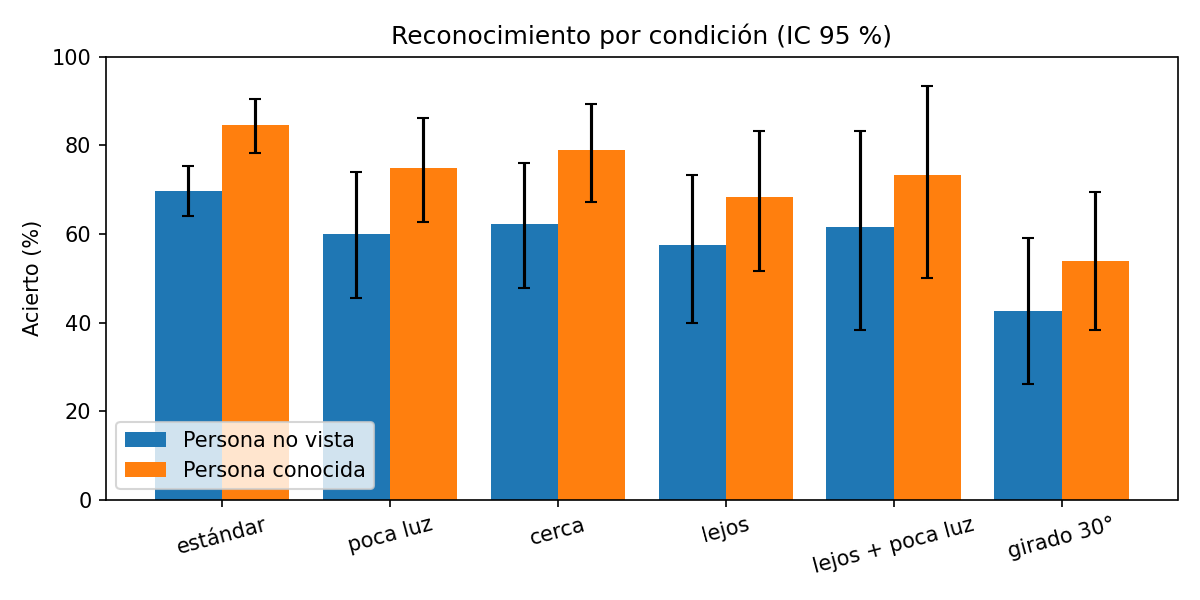
\includegraphics[width=0.95\textwidth]{robustez-por-condicion.png}
    \caption{Acierto por condición con intervalos de confianza de Wilson al 95\,\%.}
    \label{fig:robustez}
\end{figure}

La única caída cuyo intervalo de confianza al 95\,\% no incluye el cero es la del cuerpo girado 30°: $-27{,}2$ puntos (de $-44{,}5$ a $-9{,}1$) con persona no vista y $-30{,}7$ puntos (de $-48{,}0$ a $-12{,}9$) con persona conocida. Las demás condiciones caen entre 6 y 16 puntos, con intervalos que en general incluyen el cero; la excepción es «lejos» con persona conocida, cuyo intervalo termina en $-0{,}8$.

El efecto a 30° varía mucho entre personas y dispositivos: P1, con la tableta, alcanza entre 62 y 77\,\%; P2, con su teléfono, entre 22 y 29\,\%.

La detección de manos explica parte de la caída. En las señas que se realizan con las dos manos («por favor» y «¿cómo estás?»), MediaPipe detecta ambas manos en el 58,4\,\% de los cuadros en la condición estándar, pero solo en el 17,5\,\% «lejos» y en el 21,1\,\% a 30°.

Durante la grabación también se registraron los intentos de captura interrumpidos por pérdida de la mano (Tabla~\ref{tab:cortes}).

\begin{table}[h]
    \centering
    \begin{tabular}{lrrrr}
        \toprule
        Persona (dispositivo) & Poca luz & Cerca & Lejos & Girado 30° \\
        \midrule
        P1 (tableta) & 0\,\% & 0\,\% & 14\,\% & 29\,\% \\
        P2 (teléfono) & 35\,\% & 15\,\% & 22\,\% & 69\,\% \\
        P3 (teléfono) & 41\,\% & 8\,\% & --- & 52\,\% \\
        \bottomrule
    \end{tabular}
    \caption{Porcentaje aproximado de intentos de captura interrumpidos por pérdida de la mano, por condición.}
    \label{tab:cortes}
\end{table}

\section{Aprendizaje federado}
\label{sec:res-federado}

El diseño del esquema federado se describe en el Capítulo~\ref{cap:federado}. Esta sección presenta cuatro grupos de resultados: la simulación con las tres personas, el costo del entrenamiento en el dispositivo, el piloto con dispositivos reales y las medidas de protección de las actualizaciones.

\subsection{Simulación con personas reales}

La simulación entrena de forma federada solo la cabeza del modelo (la parte final, de 13\,261 parámetros), con la parte de extracción de características congelada. Para cada persona, el modelo se entrena con las otras dos (40 rondas, dos épocas locales por ronda, cinco semillas) y se evalúa con la persona excluida.

\begin{table}[h]
    \centering
    \begin{tabular}{lr}
        \toprule
        Configuración & Acierto (\%) \\
        \midrule
        Modelo del servidor, sin federar & 46,8 $\pm$ 11,3 \\
        Una sola persona (piso) & 62,3 $\pm$ 3,7 \\
        FedAvg con dos personas & 67,0 $\pm$ 4,4 \\
        FedAvg con actualizaciones a 8 bits & 67,2 $\pm$ 4,5 \\
        Entrenamiento centralizado (techo) & 67,4 $\pm$ 5,0 \\
        \bottomrule
    \end{tabular}
    \caption{Aprendizaje federado simulado con una persona excluida (cinco semillas; el $\pm$ es sobre los quince pares de persona y semilla).}
    \label{tab:federado-simulado}
\end{table}

El modelo del servidor, del que parten todas las configuraciones, se entrenó solo con la cámara web, es decir, con tomas de P1. Por eso, sin federar, acierta el 60,9\,\% con P1 y el 42,8 y 36,6\,\% con P2 y P3: en esa fila, y en el punto de partida de las demás, P1 no es una persona nueva. Las configuraciones federadas quedan entre 66,8 y 67,7\,\% para cada una de las tres personas, por lo que la ventaja inicial de P1 no se traslada al resultado final.

FedAvg queda a 0,4 puntos del entrenamiento centralizado y alcanza el 95\,\% de ese techo en unas 10 rondas. Cuantizar las actualizaciones a 8 bits reduce la subida total de 4,24\,MB a 1,06\,MB sin pérdida de acierto. La personalización de un usuario nuevo con su primera tanda de tomas mejora 4,1 puntos en promedio, y mejora a las tres personas (7,2, 1,4 y 3,8 puntos); la de un miembro ya representado, 0,9 puntos (3,4, $-1{,}7$ y 1,0). Con solo tres personas, ninguna de las dos diferencias es estadísticamente significativa: la prueba $t$ pareada sobre la media de cada persona da $p = 0{,}14$ y $p = 0{,}60$. Las semillas no se tratan como observaciones independientes, porque repiten a las mismas personas.

\subsection{Reparto sintético IID y no IID}

La propuesta plantea evaluar el esquema en condiciones no IID. Además de la simulación con las tres personas, se repartieron las 1200 tomas de cámara web entre tres clientes de dos formas: al azar (IID) y con un reparto de Dirichlet ($\alpha = 0{,}5$), en el que cada cliente recibe un subconjunto sesgado del vocabulario (no IID). Se entrenó el modelo completo con el mismo presupuesto de épocas en todos los casos y se evaluó sobre las mismas 240 tomas, con cinco semillas. Como todas las tomas son de una misma persona, el experimento aísla el efecto del reparto y no el de la diversidad de personas.

\begin{table}[h]
    \centering
    \begin{tabular}{lr}
        \toprule
        Configuración & Acierto (\%) \\
        \midrule
        Centralizado (techo) & 93,7 $\pm$ 2,7 \\
        Un cliente IID, sin colaborar & 86,5 $\pm$ 1,9 \\
        Un cliente no IID, sin colaborar & 67,2 $\pm$ 2,3 \\
        FedAvg IID & 93,3 $\pm$ 1,4 \\
        FedAvg no IID & 89,6 $\pm$ 1,9 \\
        \bottomrule
    \end{tabular}
    \caption{FedAvg con reparto IID y no IID entre tres clientes (cinco semillas). El cliente sin colaborar es el promedio de los tres clientes de cada reparto entrenados por separado.}
    \label{tab:federado-niid}
\end{table}

Cada FedAvg se compara con un cliente sin colaborar de su mismo reparto (Tabla~\ref{tab:federado-niid}). Con el reparto no IID, colaborar eleva el acierto 22,4 puntos ($p < 0{,}001$, prueba $t$ pareada sobre las semillas): un cliente con un vocabulario sesgado es el que más gana al combinarse con otros. Con el reparto IID la mejora es de 6,8 puntos y FedAvg no se distingue del entrenamiento centralizado. La heterogeneidad cuesta 3,7 puntos frente al reparto IID ($p = 0{,}015$).

Una versión anterior de este experimento comparaba el FedAvg no IID con un cliente del reparto IID y concluía que no se distinguía de un cliente aislado. Esa comparación mezclaba dos efectos, colaborar y tener datos sesgados, y se corrigió.

\subsection{Costo del entrenamiento en el dispositivo}

En la tableta de P1 se ejecutó el entrenamiento de la cabeza en el propio dispositivo, implementado en Kotlin. Con 48 tomas de entrenamiento, cada época tarda 20,5\,ms (mediana) y diez épocas, unos 0,26\,s; el cálculo de la representación de cada toma tarda 2,9\,ms y el proceso ocupa unos 6\,MB adicionales de memoria. La actualización ocupa 53\,KB en punto flotante de 32 bits y 13\,KB cuantizada a 8 bits. El acierto antes del entrenamiento coincide con el obtenido en Python (82,8\,\%), lo que verifica la equivalencia de punta a punta entre ambas implementaciones.

\subsection{Piloto con dispositivos reales}

El esquema completo se probó en una red local, con un servidor en una computadora personal y los dispositivos conectados por Wi-Fi, sin acceso a internet. En cada ronda, cada dispositivo descarga la cabeza vigente, la entrena con sus propias tomas, envía solo la actualización cuantizada (13\,285 bytes) y, al cerrarse la ronda, descarga la versión combinada.

En la ronda con la tableta (93 tomas) y el teléfono de P2 (84 tomas), el entrenamiento local tardó 0,07\,s y 0,14\,s, respectivamente, más 0,23\,s y 0,28\,s para calcular la representación de las tomas. La cabeza que cada dispositivo descargó al final coincide, bit a bit, con la publicada por el servidor.

Tras incorporar el cifrado y los códigos de participación (Sección~\ref{sec:seguridad-federado}), se repitió una ronda con la tableta: la aplicación mostró la huella del servidor, que coincidió con la impresa por la computadora, envió su actualización con el código de participación (93 tomas, 13\,285 bytes) y descargó la cabeza combinada. El entrenamiento y el cálculo de la representación tardaron 0,11\,s y 0,33\,s.

Una ronda anterior se cerró con un solo participante por un error en el cálculo del plazo de la ronda, que contaba desde la apertura y no desde la primera actualización recibida; el error se corrigió. Otra ronda recibió una actualización no solicitada de la tableta, enviada por error durante la operación remota del piloto. Ambas rondas se conservan en el registro tal como ocurrieron.

\subsection{Persona nueva y personalización}

Para evaluar el caso en que el esquema federado debería aportar más, se entrenó un modelo sin ninguna toma de P2. Luego se realizaron cuatro rondas con dos dispositivos reales: el teléfono de P2 y la tableta de P1. La Tabla~\ref{tab:federado-sin-p2} muestra el acierto sobre tomas que nunca participan del esquema federado.

\begin{table}[h]
    \centering
    \small
    \begin{tabular}{lrrrr}
        \toprule
        Modelo & \multicolumn{2}{c}{P2} & P1 & P3 \\
        & normal & sesión 2 & sesión 2 & sesión 2 \\
        \midrule
        Sin P2 (punto de partida) & 77,3 & 59,6 & 75,0 & 66,7 \\
        Federado, 4 rondas & 81,8 & 61,7 & 81,2 & 72,2 \\
        Personalizado en la computadora & 84,5 $\pm$ 2,5 & 70,6 $\pm$ 2,3 & --- & --- \\
        Personalizado en el teléfono de P2 & 82 & 66 & --- & --- \\
        \bottomrule
    \end{tabular}
    \caption{Acierto (\%) del experimento con una persona nueva. «Normal»: 22 tomas de P2 reservadas para prueba; «sesión 2»: tomas en condiciones adversas (47 de P2). P3 no participó de las rondas.}
    \label{tab:federado-sin-p2}
\end{table}

Las rondas mejoraron el modelo compartido para las tres personas, incluida P3, que no participó, y el acierto sobre el conjunto de prueba fijo del servidor pasó de 78,8\,\% a 84,6\,\%. La mejora específica para P2 fue pequeña: dos puntos en sus tomas de la sesión~2, equivalentes a una sola toma, y con oscilaciones entre rondas. La simulación de las mismas rondas en la computadora reproduce el resultado real (81,8\,\% y 59,6\,\%), y aumentar las épocas locales de dos a ocho no lo modifica.

Ajustar la cabeza solo con las 84 tomas de P2, sin promediar con otros dispositivos, eleva su acierto en la sesión~2 a 70,6\,$\pm$\,2,3\,\%. Esta personalización local se implementó en la aplicación y, ejecutada en el teléfono de P2, tardó 0,3\,s y elevó su acierto en la sesión~2 de 62\,\% a 66\,\%. El ajuste solo con P2 también mejora a P3 (de 66,7\,\% a entre 81 y 83\,\%).

\subsection{Protección de las actualizaciones}

La propuesta plantea limitar la magnitud de las actualizaciones y comprimirlas con rotación aleatoria y cuantización. Ambas medidas se evaluaron con actualizaciones reales de las tres personas (Tabla~\ref{tab:limite}).

El límite se fijó en una norma L2 de 2,0, tres veces la mediana de las actualizaciones honestas (entre 0,68 y 0,76). Ninguna actualización honesta lo alcanza, por lo que el acierto sin ataques no cambia (80,9\,\%).

\begin{table}[h]
    \centering
    \begin{tabular}{p{8.5cm}rr}
        \toprule
        Actualización maliciosa simulada & Sin límite & Con límite \\
        \midrule
        Al azar, 50 veces la norma honesta: distancia al modelo honesto & 8,34 & 0,51 \\
        Inversa del aprendizaje, 10 veces: acierto (\%) & 71,0 & 77,6 \\
        \bottomrule
    \end{tabular}
    \caption{Efecto del límite a la norma de las actualizaciones (183 tomas que no participan del esquema federado; acierto sin ataques: 80,9\,\%).}
    \label{tab:limite}
\end{table}

La rotación aleatoria previa a la cuantización no redujo el error con estas actualizaciones: el error relativo de reconstrucción a 8 bits pasó de 1,0\,\% a 1,2\,\%, y el tamaño aumentó 243 bytes por el relleno hasta potencias de dos. Las actualizaciones de la cabeza no presentan valores extremos (el máximo es de dos a cuatro veces la raíz cuadrática media de cada tensor), que es la situación en la que la rotación resulta útil.

\subsection{Ataques y agregación robusta}
\label{sec:res-ataques}

El efecto del límite se midió en una sola ronda. Para evaluar el resto de las defensas se simularon cinco rondas, como en el dispositivo: en cada una, cada persona entrena la cabeza durante dos épocas con sus tomas de la sesión~1 y envía su actualización, y un atacante que conoce las actualizaciones honestas de la ronda envía una de cuatro tipos:

\begin{itemize}
    \item \textbf{Grande:} ruido al azar con 50 veces la norma honesta.
    \item \textbf{Invertida:} $-10$ veces la actualización honesta media, con una cantidad de tomas realista.
    \item \textbf{Peso inflado:} la misma actualización invertida, declarando un millón de tomas.
    \item \textbf{Ruido bajo el límite:} ruido con el doble de la norma honesta, que no alcanza el límite.
\end{itemize}

Las defensas se aplicaron en el mismo orden que en el servidor, y una prueba automática verifica que la cabeza resultante es la misma que publicaría el servidor. Se evaluó sobre las 131 tomas de la sesión~2, que no participan del esquema; sin federar, el acierto es de 77,1\,\%. La Tabla~\ref{tab:ataques} resume el escenario del piloto: las tres personas y un atacante.

\begin{table}[h]
    \centering
    \small
    \begin{tabular}{lrrrr}
        \toprule
        Estrategia & Sin ataque & Invertida & Peso inflado & Grande \\
        \midrule
        FedAvg sin defensas & 78,5 & 14,8 & 0,0 & 73,0 \\
        FedAvg con límite & 78,5 & 73,7 & 13,0 & 78,6 \\
        FedAvg con límite y tope de 2000 & 78,5 & 73,7 & 15,0 & 78,6 \\
        FedAvg con límite y tope de 200 & 78,5 & 73,7 & 35,0 & 78,6 \\
        Mediana o media recortada & 77,7 & 78,6 & 78,6 & 78,2 \\
        \bottomrule
    \end{tabular}
    \caption{Acierto (\%) tras cinco rondas con tres personas y un atacante (cinco semillas; desvío entre semillas de hasta 2 puntos, salvo en las celdas por debajo del 40\,\%, de hasta 6). El ataque de ruido bajo el límite no modificó el acierto en ninguna estrategia. Krum no puede utilizarse con cuatro participantes.}
    \label{tab:ataques}
\end{table}

Con un peso inflado, FedAvg colapsa en dos o tres rondas aunque se apliquen el límite y el tope, porque con tres dispositivos honestos de unas cien tomas el atacante sigue dominando el promedio. La mediana y la media recortada mantienen el acierto frente a los cuatro ataques, y sin ataques cuestan 0,8 puntos.

Se repitió el experimento con quince clientes, partiendo a cada persona en cinco, y con uno o tres atacantes (tres semillas). Con un atacante, solo el peso inflado afecta a FedAvg (entre 12 y 28\,\%). Con tres, la actualización invertida lo lleva a alrededor del 61\,\% y el peso inflado, a entre 12 y 21\,\%. La mediana, la media recortada y Krum, que en este escenario sí puede utilizarse, se mantienen entre 77,6 y 79,1\,\% en todos los casos.

El acierto varía alrededor de 10 puntos entre personas en todas las configuraciones sin colapso, frente a menos de 2 puntos entre semillas. El desvío entre semillas, que es el que habitualmente se informa, subestima la variación que experimentaría una persona concreta.

\subsection{Privacidad diferencial}
\label{sec:res-privacidad}

La privacidad diferencial central se evaluó con el mismo procedimiento de cinco rondas, sin atacantes, con un recorte $C = 0{,}7$ fijado de antemano a partir de la norma honesta mediana medida en la ronda anterior del piloto. Para observar el efecto de la cantidad de dispositivos, cada persona se partió en uno, cinco o diez clientes (Tabla~\ref{tab:privacidad}).

\begin{table}[h]
    \centering
    \begin{tabular}{rrrrr}
        \toprule
        $z$ & $\varepsilon$ (5 rondas) & 3 clientes & 15 clientes & 30 clientes \\
        \midrule
        sin DP & --- & 79,1 & 78,9 & 77,1 \\
        0,3 & 63,5 & 80,2 & 78,6 & 77,9 \\
        1 & 13,2 & 12,2 & 77,6 & 78,1 \\
        2 & 6,0 & 5,3 & 59,3 & 76,8 \\
        4 & 2,8 & 3,3 & 8,7 & 53,4 \\
        \bottomrule
    \end{tabular}
    \caption{Acierto (\%) sobre la sesión~2 con privacidad diferencial central, según el multiplicador de ruido $z$ y la cantidad de clientes (tres semillas, $\delta = 10^{-5}$).}
    \label{tab:privacidad}
\end{table}

Con las tres personas del piloto, ningún valor de $\varepsilon$ menor que 10 deja un modelo utilizable: con $z = 1$ el acierto cae al 12\,\%, y los valores de ruido que no lo afectan corresponden a $\varepsilon \geq 63$, que no ofrecen una protección significativa. Como el ruido se divide por la cantidad de dispositivos, con treinta clientes $\varepsilon = 6$ conserva el 76,8\,\%. Sin embargo, en ese escenario cada cliente tiene unas nueve tomas y el esquema sin ruido tampoco mejora el modelo inicial, por lo que el resultado indica que el ruido no lo degrada, no que el modelo siga aprendiendo. Una estimación a partir de la norma de las actualizaciones indica que se necesitarían del orden de miles de dispositivos para que el ruido correspondiente a $\varepsilon \approx 6$ represente el 10\,\% de la señal.

\section{Rendimiento en los dispositivos}
\label{sec:res-rendimiento}

El rendimiento se midió en los tres dispositivos de las sesiones de captura durante el uso real de la aplicación, a partir de las métricas que la propia aplicación registra por cada captura. La Tabla~\ref{tab:rendimiento} compara la versión utilizada en la segunda sesión de captura con la versión final, que incorpora dos optimizaciones: la recepción de la imagen en formato RGBA, sin pasar por compresión JPEG ni por una rotación posterior, y la ejecución de MediaPipe en la unidad de procesamiento gráfico (GPU).

\begin{table}[h]
    \centering
    \small
    \begin{tabular}{lrrrrrr}
        \toprule
        & \multicolumn{2}{c}{Preparación (ms)} & \multicolumn{2}{c}{MediaPipe (ms)} & \multicolumn{2}{c}{Cuadros por segundo} \\
        Dispositivo & antes & después & antes & después & antes & después \\
        \midrule
        Samsung Galaxy A55 & 15,5 & 5,4 & 140 & 93 & 6,3 & 9,6 \\
        OnePlus CPH2663 & 15,7 & 2,7 & 115 & 51 & 7,5 & 17,5 \\
        Lenovo TB321FU & 6,7 & 2,4 & 50 & 35 & 16,7 & 24,9 \\
        \bottomrule
    \end{tabular}
    \caption{Tiempo por cuadro (mediana) y cuadros por segundo antes y después de las optimizaciones.}
    \label{tab:rendimiento}
\end{table}

La inferencia del modelo de clasificación tarda alrededor de 1,7\,ms por seña en la tableta, por lo que la detección de manos domina el tiempo de procesamiento.

Ninguna de las dos optimizaciones se adoptó sin medir su efecto sobre los landmarks. Ambas se compararon sobre los mismos cuadros, durante el uso de la aplicación en el Galaxy A55:

\begin{itemize}
    \item GPU frente a CPU (1190 cuadros, 378 con manos): la misma cantidad de manos detectadas en el 99,7\,\% de los cuadros y una diferencia mediana en la posición de los puntos del 0,22\,\% del ancho de la imagen (0,44\,\% en el percentil 95).
    \item Imagen sin compresión frente a JPEG de calidad 80 (1057 cuadros, 318 con manos): la misma cantidad de manos en el 99,3\,\% de los cuadros y una diferencia mediana del 0,15\,\% (0,6\,\% en el percentil 95).
\end{itemize}

Otras dos alternativas se evaluaron y se descartaron. El modo de video de MediaPipe no redujo el tiempo, porque con hasta dos manos configuradas busca la segunda mano en cada cuadro. Delegar la rotación a MediaPipe devolvió los puntos en otro sistema de coordenadas sin reducir el tiempo.

\subsection{Dispositivos adicionales}

Con la versión final se midieron otros tres dispositivos, que no participaron de las sesiones de captura: dos teléfonos de gama baja de 2019 y 2020 y una tableta de gama alta (Tabla~\ref{tab:rendimiento-extra}). En cada uno se utilizó la aplicación durante alrededor de un minuto, con señas variadas, en la condición estándar.

\begin{table}[h]
    \centering
    \small
    \setlength{\tabcolsep}{4pt}
    \begin{tabular}{llrrrr}
        \toprule
        Dispositivo & Procesador, memoria & Prep. (ms) & MediaPipe (ms) & Cuadros/s & Capturas \\
        \midrule
        Galaxy A20 & Exynos 7884, 3\,GB & 13,9 & 130 & 6,6 & 13 \\
        Galaxy A31 & Helio P65, 4\,GB & 5,3 & 92 & 9,6 & 22 \\
        Galaxy Tab S7 & Snapdragon 865, 6\,GB & 24,5 & 53 & 12,1 & 20 \\
        \bottomrule
    \end{tabular}
    \caption{Tiempo por cuadro (mediana) y cuadros por segundo en los dispositivos medidos solo con la versión final.}
    \label{tab:rendimiento-extra}
\end{table}

En los tres, MediaPipe se ejecutó en la GPU, sin recurrir al procesador central. El Galaxy A31 alcanza los mismos cuadros por segundo que el Galaxy A55, un equipo más reciente. El Galaxy A20, el más antiguo, queda en 6,6 cuadros por segundo; como no llega a nueve, la aplicación captura 10 cuadros por seña en lugar de 15, de modo que cada captura dura lo mismo que en el Galaxy A31 (alrededor de 1,5\,s). En los teléfonos de gama baja la inferencia del modelo tarda unos 8\,ms, todavía muy por debajo del tiempo de detección.

En estos teléfonos, las señas de una mano se reconocieron con confianza alta. Las señas de dos manos fueron las más afectadas: cuando el detector perdía una de las manos durante la captura, la confianza caía por debajo del umbral y la aplicación no mostraba la predicción, mientras que, con las dos manos detectadas en todos los cuadros, «por favor» y «¿cómo estás?» se reconocieron con confianzas de entre 0,86 y 1,0.

En la Galaxy Tab S7 la velocidad fue adecuada, pero en la primera prueba la mayoría de las señas se clasificó como «nada» o como otra seña. El análisis de esas tomas mostró que no se trataba de un problema de la aplicación, sino del encuadre (Sección~\ref{sec:encuadre}).

Las cifras preliminares de abril, obtenidas con otra versión del pipeline, no son comparables con estas y no se informan.

\section{Funcionamiento sin conexión}
\label{sec:res-sin-conexion}

Para verificar la premisa de procesamiento local, el 1 de noviembre se usó la aplicación en la tableta Lenovo con el modo avión activado y el Wi-Fi apagado. El registro del sistema confirma que el Wi-Fi se apagó 24\,s antes de abrir la aplicación.

\begin{itemize}
    \item \textbf{Traducción de señas.} Funcionó sin conexión: la aplicación escribió y pronunció las señas reconocidas. Como en el uso con conexión, «bien» y «por favor» fueron las que más costó reconocer.
    \item \textbf{Transcripción de voz.} En la primera prueba no funcionó: la aplicación informó que faltaba el paquete de reconocimiento sin conexión, sin recurrir a internet, como se había diseñado. Instalar los paquetes de español no lo resolvió. El registro de la aplicación mostró la causa: el servicio de voz de Google solo ofrece paquetes sin conexión de español de España y de Estados Unidos, y rechaza al instante cualquier otra variante, incluida la de Argentina que la aplicación pedía por defecto. Se modificó la aplicación para que, si el reconocimiento sin conexión rechaza la variante pedida, vuelva a intentar con esos dos paquetes, siempre en el dispositivo. Con ese cambio, el 2 de noviembre la tableta transcribió correctamente una frase en modo avión; el registro del sistema confirma la desconexión de la red antes de la prueba.
\end{itemize}

El resultado confirma que la traducción de señas y la transcripción de voz funcionan sin conexión. La segunda depende de un componente del sistema operativo que debe descargarse una vez y que no existe para la variante argentina del español; la aplicación lo resuelve usando la variante de Estados Unidos para el reconocimiento, mientras que la voz que lee las señas conserva la variante elegida.

\section{Variantes del modelo exportado}
\label{sec:res-variantes}

El modelo original utilizaba operaciones de TensorFlow no incluidas en el núcleo de TensorFlow Lite (\emph{Flex}), que obligaban a incluir en la aplicación una biblioteca de 169,4\,MB. Al reexportar el modelo con las capas LSTM desenrolladas en operaciones básicas, la aplicación dejó de necesitar esa biblioteca y su tamaño pasó de 243,5\,MB a 67,4\,MB ($-72$\,\%).

\begin{table}[h]
    \centering
    \begin{tabular}{lrr}
        \toprule
        Variante sin operaciones Flex & Tamaño (KB) & Coincide con Keras (\%) \\
        \midrule
        Punto flotante de 32 bits & 701 & 100 \\
        Cuantización dinámica (adoptada) & 236 & 100 \\
        Cuantización entera de 8 bits & 276 & 99,7 \\
        \bottomrule
    \end{tabular}
    \caption{Variantes del modelo exportado sin operaciones Flex.}
    \label{tab:variantes}
\end{table}

La exportación con la capa LSTM fusionada de TensorFlow~2.10 producía resultados incorrectos (coincidía con Keras solo en el 51\,\% de las predicciones), por lo que se adoptó la versión desenrollada. El modelo final publicado en la aplicación, en su variante con cuantización dinámica, ocupa 236\,KB y coincide con Keras en el 99,9\,\% de las predicciones.
